\documentclass{beamer}
\usepackage[utf8]{inputenc}
\usepackage{graphicx, epsfig}
\usepackage{amsmath,mathrsfs,amsfonts,amssymb}
\usepackage{floatflt}
\usepackage{epic,ecltree}
\usepackage{mathtext}
\usepackage{fancybox}
\usepackage{fancyhdr}
\usepackage{multirow}
\usepackage{enumerate}
\usepackage{epstopdf}
\usepackage{multicol}
\usepackage{algorithm}
\usepackage[noend]{algorithmic}
\usepackage{tikz}
\usepackage{blindtext}
\usetheme{default}%{Singapore}%{Warsaw}%{Warsaw}%{Darmstadt}
\usecolortheme{default}

\setbeamerfont{title}{size=\Huge}
\setbeamertemplate{footline}[page number]{}

\setbeamertemplate{section in toc}[sections numbered]


\makeatletter
\newcommand\HUGE{\@setfontsize\Huge{35}{40}}
\makeatother    

\setbeamerfont{title}{size=\HUGE}
\beamertemplatenavigationsymbolsempty

% latin bold lower
\newcommand{\ba}{\mathbf{a}} 
\newcommand{\bc}{\mathbf{c}} 
\newcommand{\be}{\mathbf{e}} 
\newcommand{\bh}{\mathbf{h}} 
\newcommand{\bp}{\mathbf{p}} 
\newcommand{\bt}{\mathbf{t}} 
\newcommand{\bs}{\mathbf{s}} 
\newcommand{\bu}{\mathbf{u}} 
\newcommand{\bv}{\mathbf{v}} 
\newcommand{\bw}{\mathbf{w}} 
\newcommand{\bx}{\mathbf{x}} 
\newcommand{\by}{\mathbf{y}} 
\newcommand{\bz}{\mathbf{z}} 

% latin bold upper
\newcommand{\bA}{\mathbf{A}} 
\newcommand{\bB}{\mathbf{B}} 
\newcommand{\bC}{\mathbf{C}} 
\newcommand{\bI}{\mathbf{I}} 
\newcommand{\bJ}{\mathbf{J}} 
\newcommand{\bL}{\mathbf{L}} 
\newcommand{\bM}{\mathbf{M}} 
\newcommand{\bP}{\mathbf{P}}
\newcommand{\bQ}{\mathbf{Q}} 
\newcommand{\bR}{\mathbf{R}} 
\newcommand{\bT}{\mathbf{T}} 
\newcommand{\bU}{\mathbf{U}} 
\newcommand{\bV}{\mathbf{V}} 
\newcommand{\bW}{\mathbf{W}} 
\newcommand{\bX}{\mathbf{X}} 
\newcommand{\bY}{\mathbf{Y}} 
\newcommand{\bZ}{\mathbf{Z}} 

% latin cal upper
\newcommand{\cF}{\mathcal{F}} 
\newcommand{\cG}{\mathcal{G}} 
\newcommand{\cI}{\mathcal{I}} 
\newcommand{\cL}{\mathcal{L}} 
\newcommand{\cM}{\mathcal{M}} 
\newcommand{\cN}{\mathcal{N}} 
\newcommand{\cP}{\mathcal{P}} 
\newcommand{\cS}{\mathcal{S}} 
\newcommand{\cT}{\mathcal{T}} 
\newcommand{\cW}{\mathcal{W}} 
\newcommand{\cX}{\mathcal{X}} 
\newcommand{\cZ}{\mathcal{Z}} 

% latin bb upper
\newcommand{\bbE}{\mathbb{E}} 
\newcommand{\bbI}{\mathbb{I}} 
\newcommand{\bbP}{\mathbb{P}} 
\newcommand{\bbR}{\mathbb{R}} 

% greek bold lower
\newcommand{\bepsilon}{\boldsymbol{\epsilon}} 
\newcommand{\btheta}{\boldsymbol{\theta}} 
\newcommand{\blambda}{\boldsymbol{\lambda}} 
\newcommand{\bpi}{\boldsymbol{\pi}} 
\newcommand{\bmu}{\boldsymbol{\mu}} 
\newcommand{\bsigma}{\boldsymbol{\sigma}} 
\newcommand{\bphi}{\boldsymbol{\phi}} 

% greek bold upper
\newcommand{\bSigma}{\boldsymbol{\Sigma}} 

\DeclareMathOperator*{\argmin}{arg\,min}
\DeclareMathOperator*{\argmax}{arg\,max}

\newcommand{\createdgmtitle}[1]{\title[\hbox to 56mm{Deep Generative Models  \hfill\insertframenumber\,/\,\inserttotalframenumber}]
	{\vspace{1cm} \\ \textbf{Deep Generative Models} \\ {\Huge Lecture #1}}
	\author{Roman Isachenko}
		\institute{
\includegraphics[width=0.7cm]{../utils/aimasterslogo} \LARGE{AI Masters}}
	\date{2024, Spring}
}

\usepackage{tikz}
\usetikzlibrary{arrows,shapes,positioning,shadows,trees}

\newcommand\myfootnote[1]{%
  \tikz[remember picture,overlay]
  \draw (current page.south west) +(1in + \oddsidemargin,0.5em)
  node[anchor=south west,inner sep=0pt]{\parbox{\textwidth}{%
      \rlap{\rule{10em}{0.4pt}}\raggedright\scriptsize \textit{#1}}};}

\newcommand\myfootnotewithlink[2]{%
  \tikz[remember picture,overlay]
  \draw (current page.south west) +(1in + \oddsidemargin,0.5em)
  node[anchor=south west,inner sep=0pt]{\parbox{\textwidth}{%
      \rlap{\rule{10em}{0.4pt}}\raggedright\scriptsize\href{#1}{\textit{#2}}}};}
      
\AtBeginSection[]
      {
      	\begin{frame}{Outline}
      		\tableofcontents[currentsection]
      	\end{frame}
      }
      \AtBeginSubsection[]{
      	\begin{frame}{Outline}
      		\tableofcontents[currentsection,currentsubsection]
      	\end{frame}
}
\createdgmtitle{12}

\usepackage{tikz}

\usetikzlibrary{arrows,shapes,positioning,shadows,trees}
%--------------------------------------------------------------------------------
\begin{document}
%--------------------------------------------------------------------------------
\begin{frame}[noframenumbering,plain]
%\thispagestyle{empty}
\titlepage
\end{frame}
%=======
\begin{frame}{Recap of previous lecture}
	\begin{block}{Langevin dynamic}
		\vspace{-0.3cm}
		\[
			\bx_{l + 1} = \bx_l + \frac{\eta}{2} \cdot \nabla_{\bx_l} \log p(\bx_l | \btheta) + \sqrt{\eta} \cdot \bepsilon, \quad \bepsilon \sim \cN(0, \bI).
		\]
		\vspace{-0.7cm}
	\end{block}
	\begin{block}{Fisher divergence}
		\vspace{-0.3cm}
		\[
			D_F(\pi, p) = \frac{1}{2}\bbE_{\pi}\bigl\| \nabla_{\bx}\log p(\bx| \btheta) - \nabla_\bx \log \pi(\bx) \bigr\|^2_2 \rightarrow \min_{\btheta}
		\]
		\vspace{-0.7cm}
	\end{block}
	\begin{block}{Score function}
		\vspace{-0.5cm}
		 \[
			 \bs_{\btheta}(\bx) = \nabla_{\bx}\log p(\bx| \btheta)
		 \]
	 \vspace{-0.8cm}
	\end{block}
	\begin{figure}
		\centering
		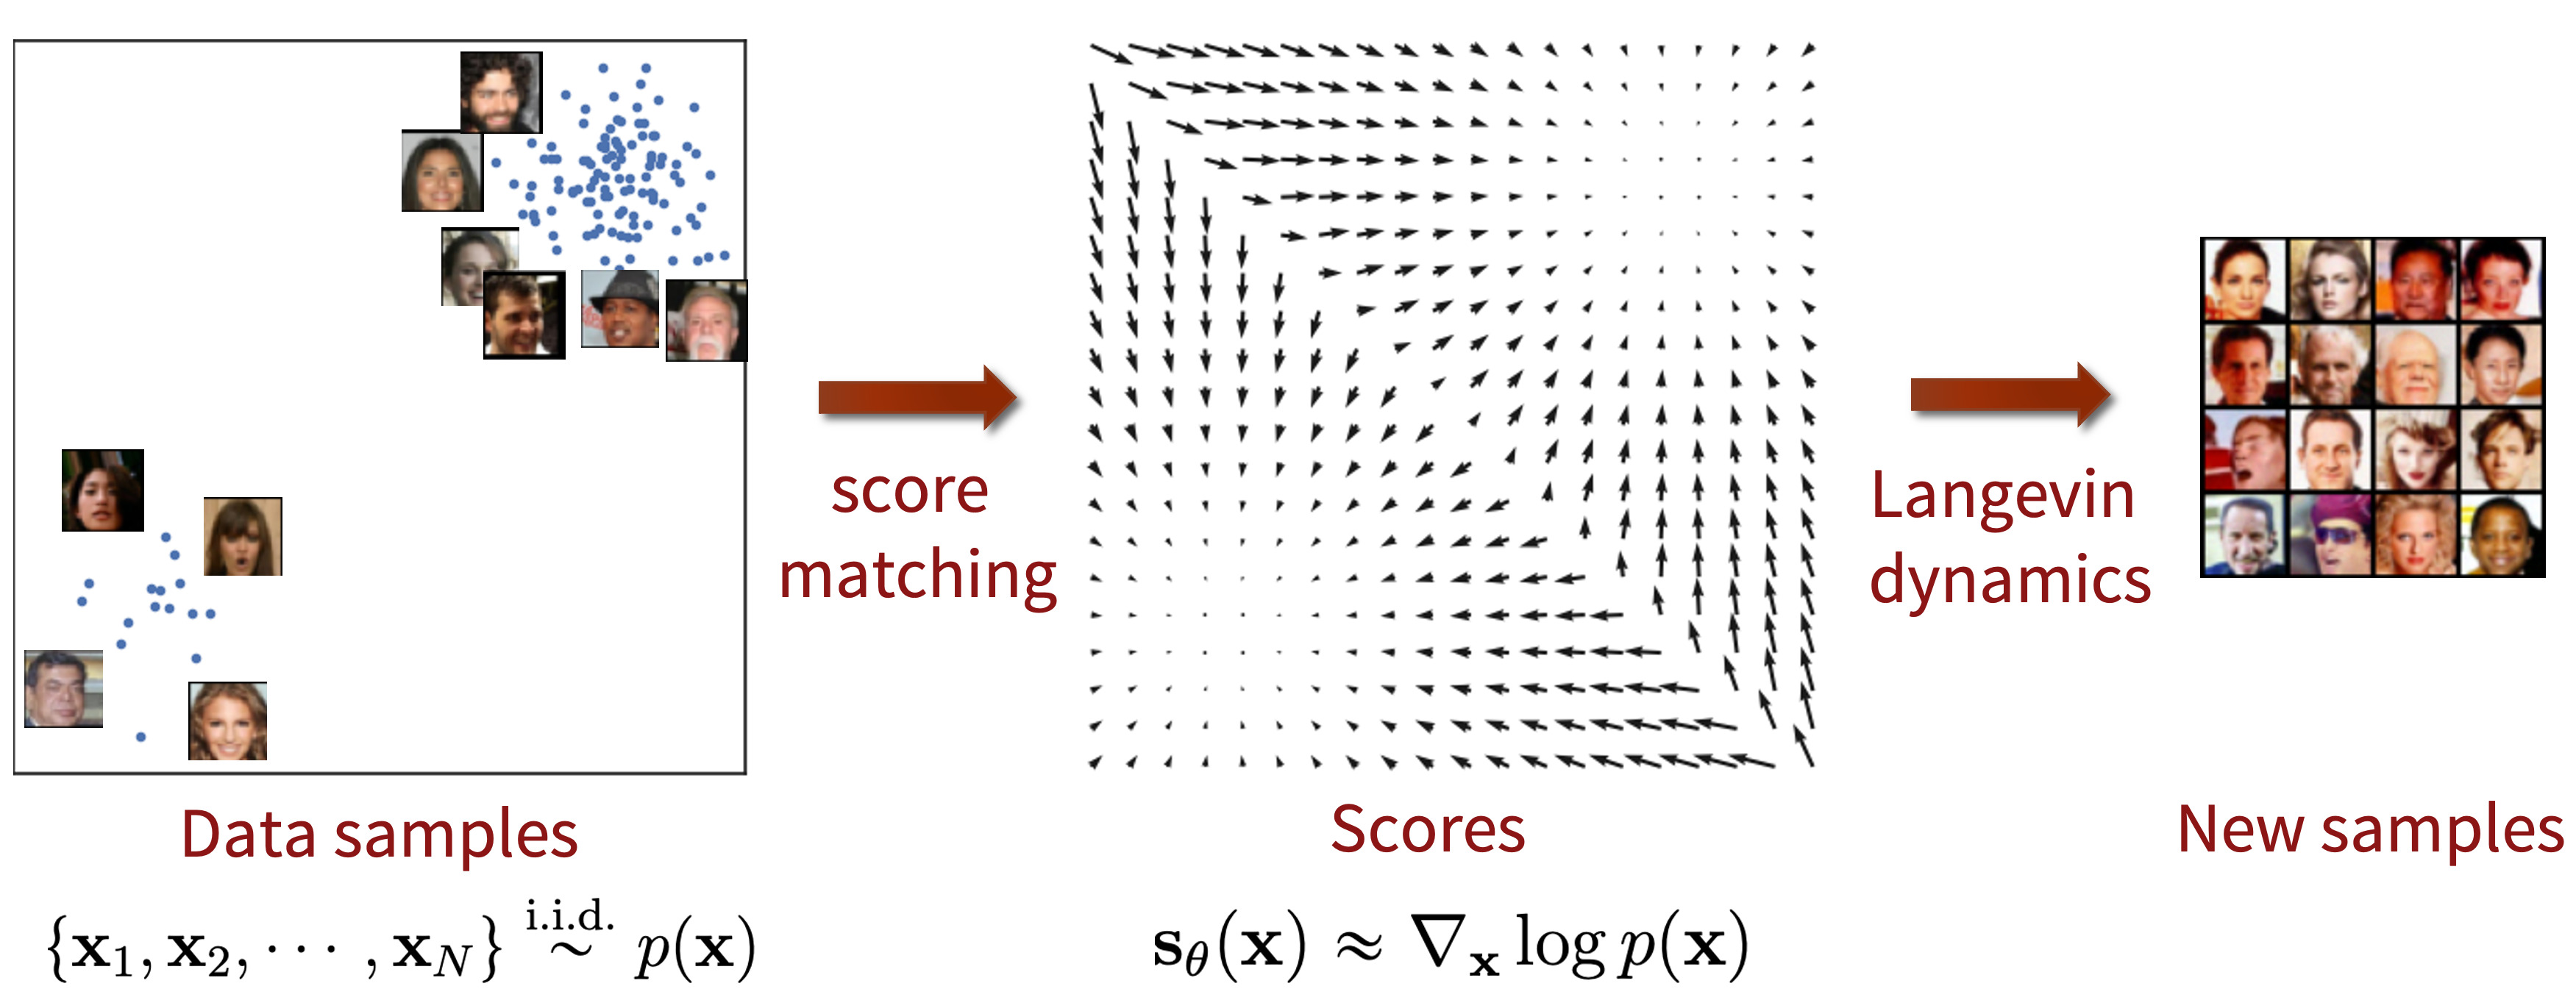
\includegraphics[width=0.75\linewidth]{figs/smld}
	\end{figure}
	\myfootnotewithlink{https://yang-song.github.io/blog/2021/score/}{Song Y. Generative Modeling by Estimating Gradients of the Data Distribution, blog post, 2021}
\end{frame}
%=======
\begin{frame}{Recap of previous lecture}
	Let perturb original data by normal noise $q(\bx' | \bx, \sigma) = \cN(\bx, \sigma^2 \bI)$
	\vspace{-0.3cm}
	\[
	\pi(\bx' | \sigma) = \int \pi(\bx) q(\bx' | \bx, \sigma) d\bx.
	\]
	\vspace{-0.6cm} \\
	Then the solution of 
	\vspace{-0.2cm}
	\[
	\frac{1}{2} \bbE_{\pi(\bx' | \sigma)}\bigl\| \bs_{\btheta}(\bx', \sigma) - \nabla_{\bx'} \log \pi(\bx' | \sigma) \bigr\|^2_2 \rightarrow \min_{\btheta}
	\]
	\vspace{-0.5cm} \\
	satisfies $\bs_{\btheta}(\bx', \sigma) \approx \bs_{\btheta}(\bx', 0) = \bs_{\btheta}(\bx')$ if $\sigma$ is small enough.
	\begin{block}{Theorem (denoising score matching)}
		\vspace{-0.8cm}
		\begin{multline*}
			\bbE_{\pi(\bx' | \sigma)}\bigl\| \bs_{\btheta}(\bx', \sigma) - \nabla_{\bx'} \log \pi(\bx' | \sigma) \bigr\|^2_2 = \\ = \bbE_{\pi(\bx)} \bbE_{q(\bx' | \bx, \sigma)}\bigl\| \bs_{\btheta}(\bx', \sigma) - \nabla_{\bx'} \log q(\bx' | \bx, \sigma) \bigr\|^2_2 + \text{const}(\btheta)
		\end{multline*}
		\vspace{-0.8cm}
	\end{block}
	Here $\nabla_{\bx'} \log q(\bx' | \bx, \sigma) = - \frac{\bx' - \bx}{\sigma^2}$.
	\begin{itemize}
		\item The RHS does not need to compute $\nabla_{\bx'} \log \pi(\bx' | \sigma)$ and even more $\nabla_{\bx'} \log \pi(\bx')$.
		\item $\bs_{\btheta}(\bx', \sigma)$ tries to \textbf{denoise} a corrupted sample.
		\item Score function $\bs_{\btheta}(\bx', \sigma)$ parametrized by $\sigma$. 
	\end{itemize}
	\myfootnotewithlink{http://www.iro.umontreal.ca/~vincentp/Publications/smdae_techreport.pdf}{Vincent P. A Connection Between Score Matching and Denoising Autoencoders, 2010}
\end{frame}
%=======
\begin{frame}{Recap of previous lecture}
	\begin{block}{Noise conditioned score network}
		\begin{itemize}
			\item Define the sequence of noise levels: $\sigma_1 > \sigma_2 > \dots > \sigma_T$.
			\item Train denoised score function $\bs_{\btheta}(\bx', \sigma)$ for each noise level:
			\vspace{-0.3cm}
			\[
				\sum_{t=1}^T {\color{violet}\sigma_t^2} \bbE_{\pi(\bx)} \bbE_{q(\bx' | \bx, \sigma_t)}\bigl\| \bs_{\btheta}(\bx', \sigma_t) - \nabla_\bx' \log q(\bx' | \bx, \sigma_t) \bigr\|^2_2 \rightarrow \min_{\btheta}
			\]
			\vspace{-0.5cm}
			\item Sample from \textbf{annealed} Langevin dynamics (for $t=1, \dots, T$).
		\end{itemize}
	\end{block}
	\begin{figure}
		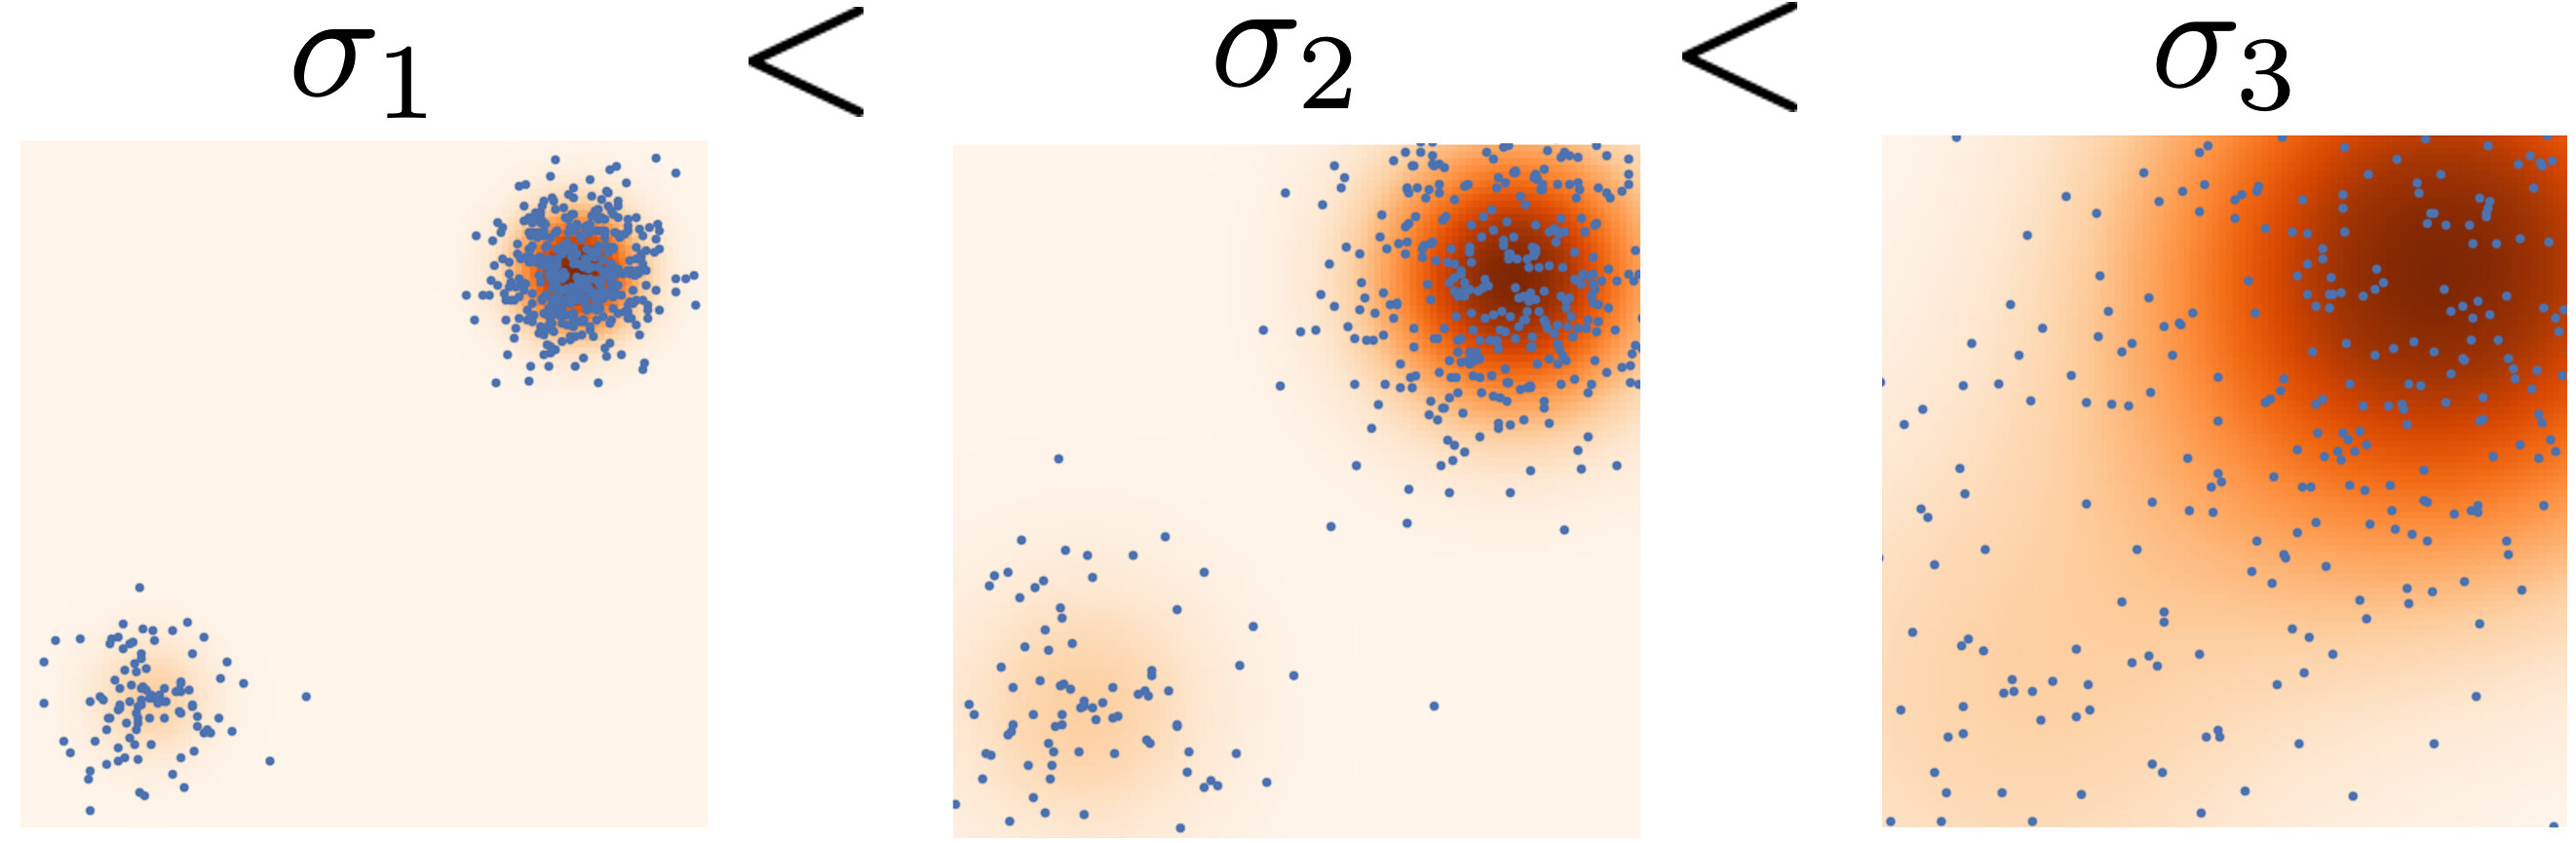
\includegraphics[width=0.55\linewidth]{figs/multi_scale}
	\end{figure}
	\begin{figure}
		
\includegraphics[width=\linewidth]{figs/duoduo}
	\end{figure}
	\myfootnotewithlink{https://arxiv.org/abs/1907.05600}{Song Y. et al. Generative Modeling by Estimating Gradients of the Data Distribution, 2019}
\end{frame}
%=======
\begin{frame}{Recap of previous lecture}
	\begin{block}{NCSN training}
		\begin{enumerate}
			\item Get the sample $\bx_0 \sim \pi(\bx)$.
			\item Sample noise level $t \sim U[1, T]$ and the noise $\bepsilon \sim \cN(0, \bI)$.
			\item Get noisy image $\bx' = \bx_0 + \sigma_t \cdot \bepsilon$.
			\item Compute loss $ \cL = \| \bs_{\btheta}(\bx', \sigma_t) + \frac{\bepsilon}{\sigma_t} \|^2 $.
		\end{enumerate}
	\end{block}
	\begin{block}{NCSN sampling (annealed Langevin dynamics)}
		\begin{itemize}
			\item Sample $\bx_0 \sim \cN(0, \sigma_1 \bI) \approx \pi(\bx | \sigma_1)$.
			\item Apply $T$ steps of Langevin dynamic
			\vspace{-0.2cm}
			\[
				\bx_l = \bx_{l-1} + \frac{\eta_t}{2} \cdot \bs_{\btheta}(\bx_{l - 1}, \sigma_t) + \sqrt{\eta_t} \cdot \bepsilon_l.
			\] 
			\vspace{-0.5cm}
			\item Update $\bx_0 := \bx_L$ and choose the next $\sigma_t$.
		\end{itemize}
	\end{block}
	\myfootnotewithlink{https://arxiv.org/abs/2006.09011}{Song Y. et al. Improved Techniques for Training Score-Based Generative Models, 2020}
\end{frame}
%=======
\begin{frame}{Outline}
	\tableofcontents
\end{frame}
%=======
\section{Gaussian diffusion process}
%=======
\subsection{Forward gaussian diffusion process}
%=======
\begin{frame}{Forward gaussian diffusion process}
	Let $\bx_0 = \bx \sim \pi(\bx)$, $\beta_t \in (0, 1)$. Define the Markov chain
	\[
		\bx_t = \sqrt{1 - \beta_t} \cdot \bx_{t - 1} + \sqrt{\beta_t} \cdot \bepsilon, \quad \text{where }\bepsilon \sim \cN(0, \bI);
	\]
	\[
		q(\bx_t | \bx_{t-1}) = \cN(\sqrt{1 - \beta_t} \cdot \bx_{t-1}, \beta_t \cdot \bI).
	\]
	\vspace{-0.5cm}
	\begin{block}{Statement 1}
		Let denote $\alpha_t = 1 - \beta_t$ and $\bar{\alpha}_t = \prod_{s=1}^t \alpha_s$. Then
		\[
			q(\bx_t | \bx_0) = \cN(\sqrt{\bar{\alpha}_t} \cdot \bx_0, (1 - \bar{\alpha}_t) \cdot \bI)
		\]
		We are able to sample from any timestamp using only $\bx_0$!
		\vspace{-0.2cm}
		{\small
		\begin{multline*}
			\bx_t = \sqrt{\alpha_t} \cdot {\color{teal}\bx_{t-1}} + \sqrt{1 - \alpha_t} \cdot \boldsymbol{\epsilon}_t = \\
			= \sqrt{\alpha_t} ({\color{teal} \cdot \sqrt{\alpha_{t-1}} \bx_{t-2} + \sqrt{1 - \alpha_{t-1}} \cdot  \boldsymbol{\epsilon}_{t-1}}) + \sqrt{1 - \alpha_t} \cdot \boldsymbol{\epsilon}_t = \\
			= \sqrt{\alpha_t \alpha_{t-1}} \cdot \bx_{t-2} + ( {\color{violet}\sqrt{\alpha_t (1 - \alpha_{t-1})} \cdot  \boldsymbol{\epsilon}_{t-1} + \sqrt{1 - \alpha_t} \cdot \boldsymbol{\epsilon}_t}) = \\
			= \sqrt{\alpha_t \alpha_{t-1}} \cdot \bx_{t-2} + {\color{violet}\sqrt{1 - \alpha_{t-1} \alpha_t} \cdot \boldsymbol{\epsilon}'_t} = \\
			 = \dots = \sqrt{\bar{\alpha}_t} \cdot \bx_{0} + \sqrt{1 - \bar{\alpha}_t} \cdot \bepsilon, \quad \text{where } \bepsilon \sim \cN(0, \bI).
		\end{multline*}
		}
	\end{block}
	\myfootnotewithlink{http://proceedings.mlr.press/v37/sohl-dickstein15.pdf}{Sohl-Dickstein J. Deep Unsupervised Learning using Nonequilibrium Thermodynamics, 2015}
 \end{frame}
%=======
\begin{frame}{Forward gaussian diffusion process}
	\vspace{-0.5cm}
	\begin{align*}
		q(\bx_t | \bx_{t-1}) &= \cN\left(\sqrt{1 - \beta_t} \cdot \bx_{t-1}, \beta_t \cdot \bI\right); \\
		q(\bx_t | \bx_0) &= \cN\left(\sqrt{\bar{\alpha}_t} \cdot \bx_0, (1 - \bar{\alpha}_t) \cdot \bI\right).
	\end{align*}
	At each step we
	\begin{itemize}
		\item scale magnitude of the signal at rate $\sqrt{1 - \beta_t}$;
		\item add noise with variance $\beta_t$.
	\end{itemize}
	\begin{block}{Statement 2}
		Applying the Markov chain to samples from any $\pi(\bx)$ we will get $\bx_{\infty} \sim p_{\infty}(\bx) = \cN(0, \bI)$. Here $p_{\infty}(\bx)$ is a \textbf{stationary} and \textbf{limiting} distribution:
		\vspace{-0.2cm}
		\[
			p_{\infty}(\bx) = \int q(\bx | \bx') p_{\infty}(\bx') d \bx'. 
		\]
		\[
			p_{\infty}(\bx) = \int q(\bx_{\infty} | \bx_0) \pi(\bx_0) d\bx_0 \approx \cN(0, \bI) \int \pi(\bx_0) d\bx_0 = \cN(0, \bI)
		\]
		\vspace{-0.8cm}
	\end{block}
	\myfootnotewithlink{http://proceedings.mlr.press/v37/sohl-dickstein15.pdf}{Sohl-Dickstein J. Deep Unsupervised Learning using Nonequilibrium Thermodynamics, 2015}
 \end{frame}
%=======
\begin{frame}{Forward gaussian diffusion process}
	\textbf{Diffusion} refers to the flow of particles from high-density regions towards low-density regions.
	\vspace{-0.2cm}
	\begin{figure}
		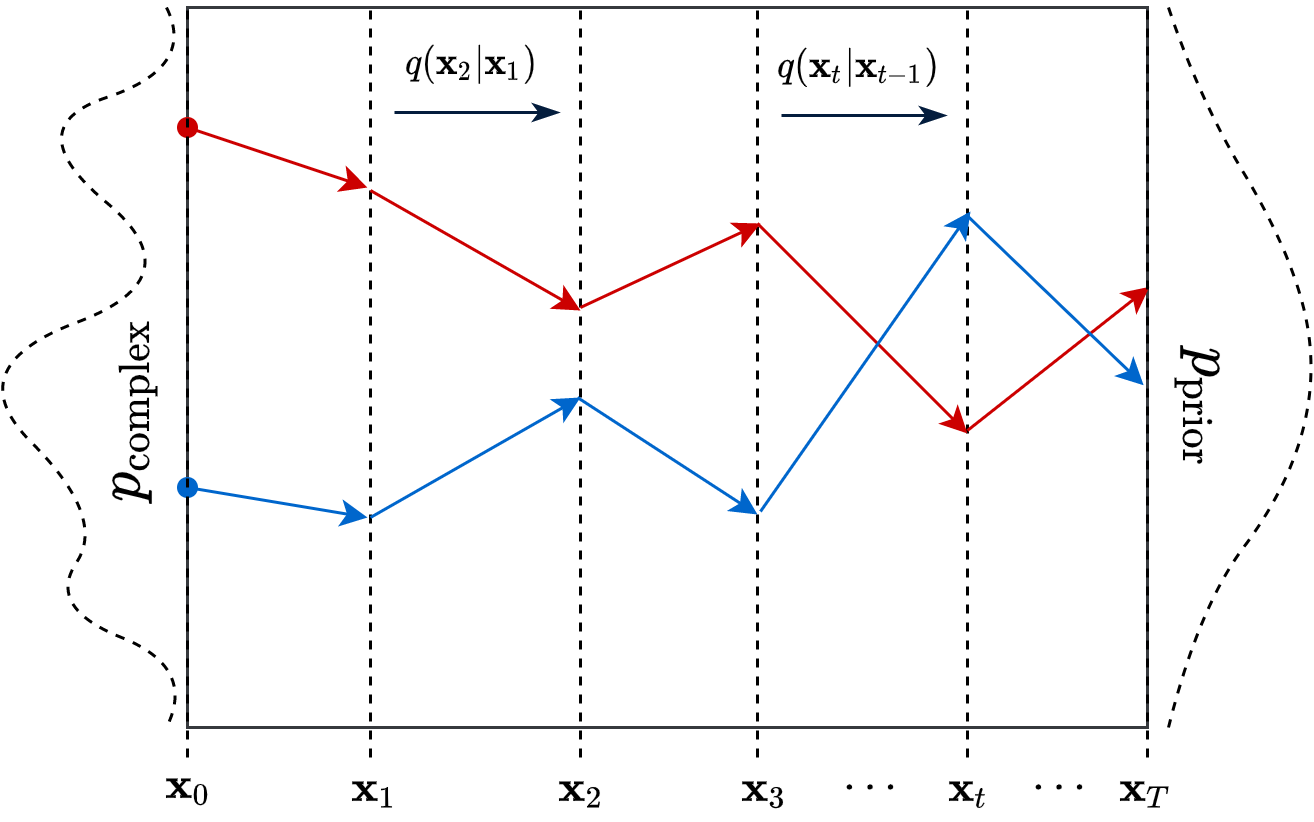
\includegraphics[width=0.5\linewidth]{figs/diffusion_over_time}
	\end{figure}
	\vspace{-0.6cm}
	\begin{enumerate}
		\item $\bx_0 = \bx \sim \pi(\bx)$;
		\item $\bx_t = \sqrt{1 - \beta_t} \cdot \bx_{t - 1} + \sqrt{\beta_t} \cdot \bepsilon$, where $\bepsilon \sim \cN(0, \bI)$, $t \geq 1$;
		\item $\bx_T \sim p_{\infty}(\bx) = \cN(0, \bI)$, where $T >> 1$.
	\end{enumerate}
	If we are able to invert this process, we will get the way to sample $\bx \sim \pi(\bx)$ using noise samples $p_{\infty}(\bx) = \cN(0, \mathbf{I})$. \\ 
	Now our goal is to revert this process.
	\myfootnotewithlink{https://ayandas.me/blog-tut/2021/12/04/diffusion-prob-models.html}{Das A. An introduction to Diffusion Probabilistic Models, blog post, 2021}
\end{frame}
%=======
\subsection{Denoising score matching}
%=======
\begin{frame}{Denoising score matching}
	\begin{block}{NCSN} 
		\[
			\quad q(\bx_t | \bx_0) = \cN(\bx, \sigma_t^2 \bI)
		\]
		\[
			\pi(\bx' | \sigma_1) \approx \cN(0, \sigma_1^2 \bI), \quad \pi(\bx' | \sigma_T) \approx \pi(\bx).
		\]
	\end{block}
	\begin{block}{Gaussian diffussion}
	\[
		q(\bx_t | \bx_0) = \cN(\sqrt{\bar{\alpha}_t} \cdot \bx_0, (1 - \bar{\alpha}_t) \cdot \bI).
	\]
	\[
		q(\bx_1) \approx \pi(\bx), \quad q(\bx_T) \approx \cN(0, \bI).
	\]
	\end{block}
	\vspace{-0.4cm} 
	\begin{block}{Theorem}
	\vspace{-0.5cm}
	\begin{multline*}
		\bbE_{\pi(\bx' | \sigma)}\bigl\| \bs_{\btheta}(\bx', \sigma) - \nabla_{\bx'} \log \pi(\bx' | \sigma) \bigr\|^2_2 = \\
		= \bbE_{\pi(\bx)} \bbE_{q(\bx' | \bx, \sigma)}\bigl\| \bs_{\btheta}(\bx', \sigma) - \nabla_{\bx'} \log q(\bx' | \bx, \sigma) \bigr\|^2_2 + \text{const}(\btheta)
	\end{multline*}
	\vspace{-0.5cm}
	\end{block}
	\begin{block}{Gradient of the noise kernel}
		\vspace{-0.4cm}
		\[
			\nabla_{\bx'} \log q(\bx' | \bx, \sigma) = \nabla_{\bx'} \log \cN(\bx, \sigma^2 \bI) = - \frac{\bx' - \bx}{\sigma^2}
		\]
		\vspace{-0.5cm}
	\end{block}
	\myfootnotewithlink{http://www.iro.umontreal.ca/~vincentp/Publications/smdae_techreport.pdf}{Vincent P. A Connection Between Score Matching and Denoising Autoencoders, 2010}
\end{frame}
%=======
\subsection{Reverse gaussian diffusion process}
%=======
\begin{frame}{Reverse gaussian diffusion process}
	\begin{figure}
		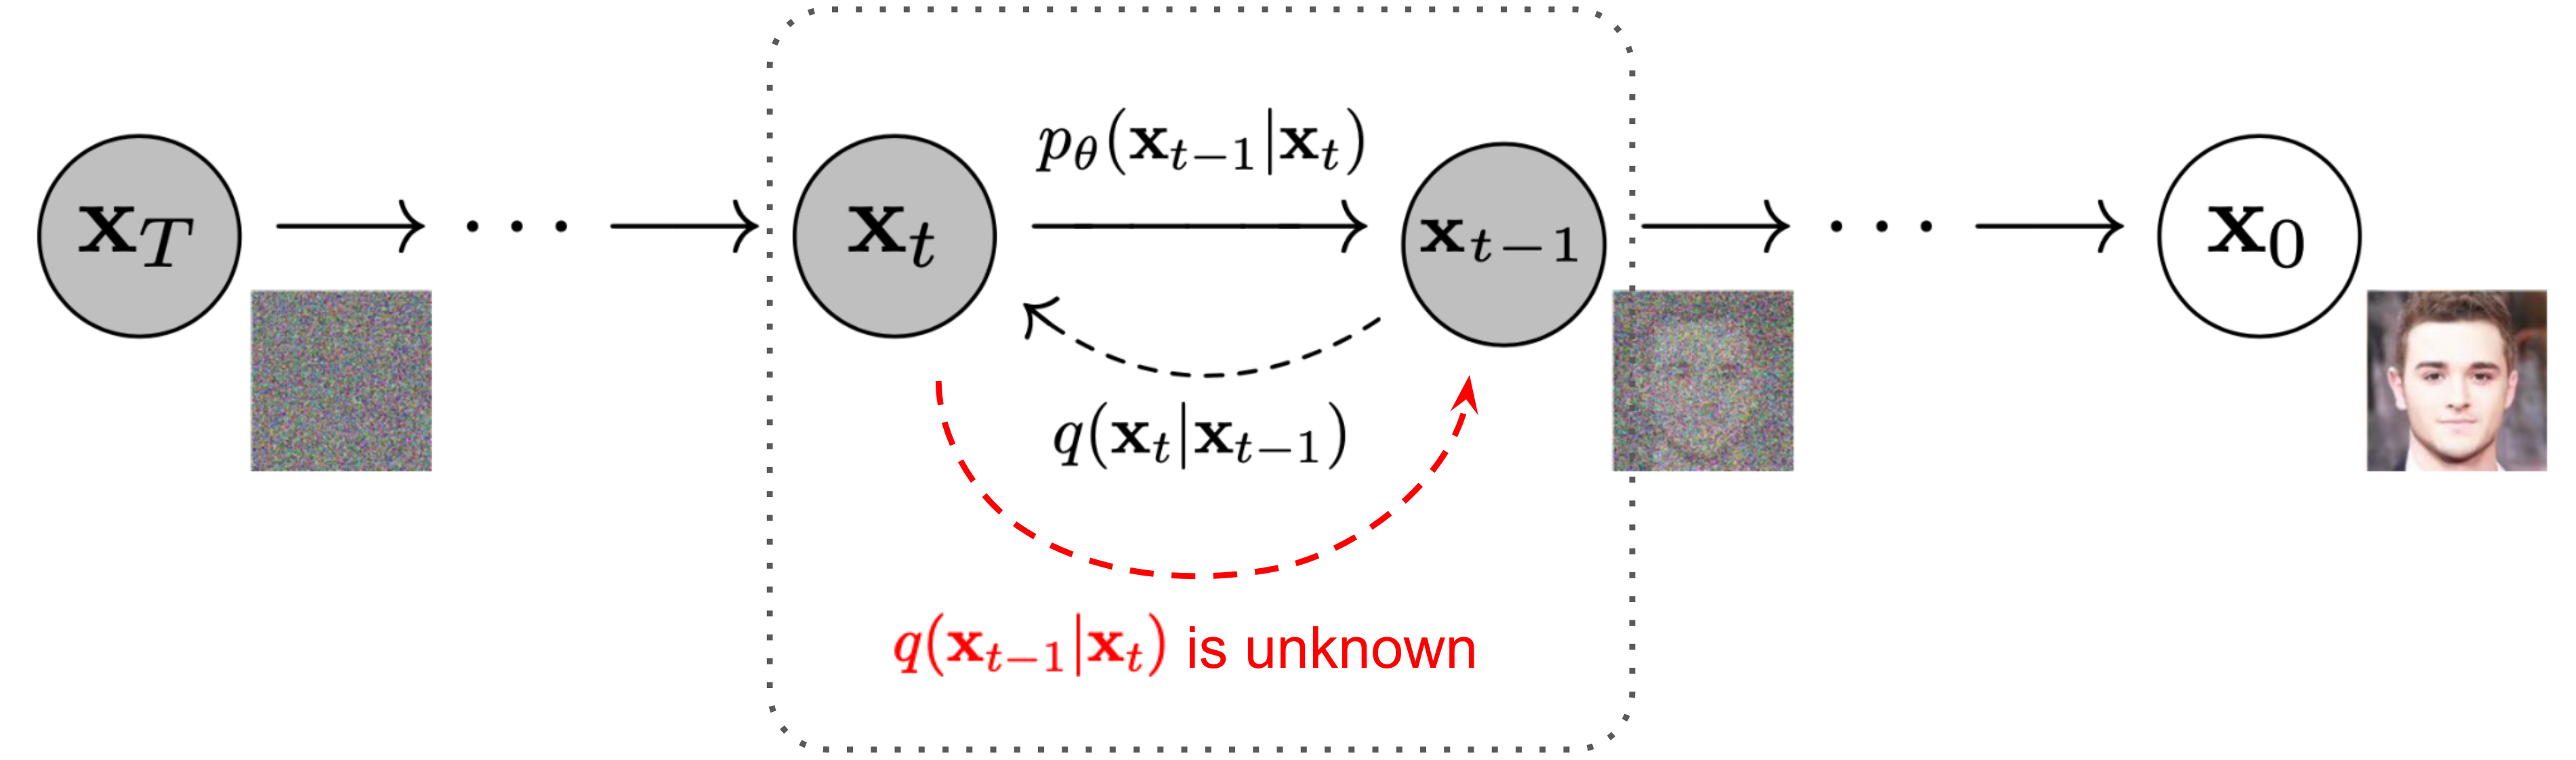
\includegraphics[width=0.8\linewidth]{figs/DDPM}
	\end{figure}
	\vspace{-0.5cm}
	\begin{block}{Forward process}
		\vspace{-0.3cm}
		\[
			q(\bx_t | \bx_{t-1}) = \cN\left(\sqrt{1 - \beta_t} \cdot \bx_{t-1}, \beta_t \cdot \bI\right).
		\]
		\vspace{-0.5cm}
	\end{block}
	\begin{block}{Reverse process}
		\vspace{-0.3cm}
		\[
			q(\bx_{t-1}|\bx_{t}) = \frac{q(\bx_{t}|\bx_{t-1}) {\color{violet}q(\bx_{t-1})}}{{\color{violet}q(\bx_{t})}} \approx p(\bx_{t - 1} | \bx_t, \btheta)
		\]
		\vspace{-0.3cm}
		\begin{itemize}
			\item ${\color{violet}q(\bx_{t-1})}$, ${\color{violet}q(\bx_{t})}$ are intractable.
			\item If $\beta_t$ is small enough, $q(\bx_{t-1}|\bx_{t})$ will be Gaussian (Feller, 1949).
		\end{itemize}
	\end{block}
	\myfootnotewithlink{}{Feller W. On the theory of stochastic processes, with particular reference to applications, 1949}
	\end{frame}
%=======
\begin{frame}{Reverse gaussian diffusion process}
		\vspace{-0.4cm}
		\begin{align*}
			q(\bx_{t-1}|\bx_{t}) &= \frac{q(\bx_{t}|\bx_{t-1}) {\color{violet}q(\bx_{t-1})}}{{\color{violet}q(\bx_{t})}} \\
			q(\bx_{t-1}|\bx_{t}, {\color{olive}\bx_0}) &= \frac{q(\bx_{t}|\bx_{t-1}, {\color{olive}\bx_0}) q(\bx_{t-1} | {\color{olive}\bx_0}) }{q(\bx_{t}| {\color{olive}\bx_0})} = \cN(\tilde{\bmu}_t(\bx_t, \bx_0), \tilde{\beta}_t \bI)
		\end{align*}
		\vspace{-0.2cm}
		\begin{itemize}
			\item ${\color{violet}q(\bx_{t-1})}$, ${\color{violet}q(\bx_{t})}$ are intractable.
			\item If $\beta_t$ is small enough, $q(\bx_{t-1}|\bx_{t})$ will be Gaussian (Feller, 1949).
		\end{itemize}
	\vspace{-0.2cm}
	\begin{figure}
		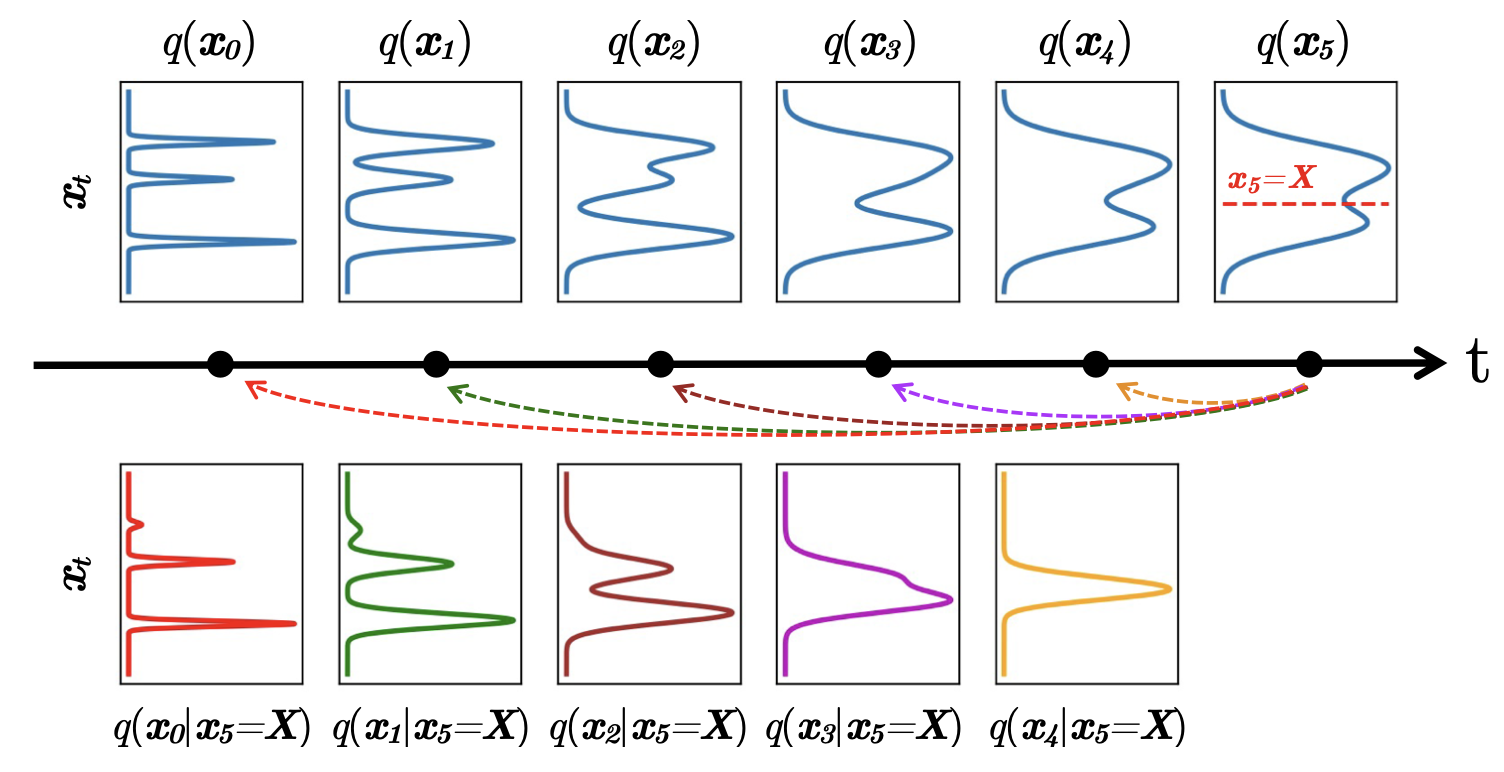
\includegraphics[width=0.7\linewidth]{figs/inverse_distr_1d}
	\end{figure}
	\myfootnotewithlink{https://arxiv.org/abs/2112.07804}{Xiao Z., Kreis K., Vahdat A. Tackling the generative learning trilemma with denoising diffusion GANs, 2021}
	\end{frame} 
%=======
\begin{frame}{Reverse gaussian diffusion process}
	\vspace{-0.3cm} 
	\begin{figure}
		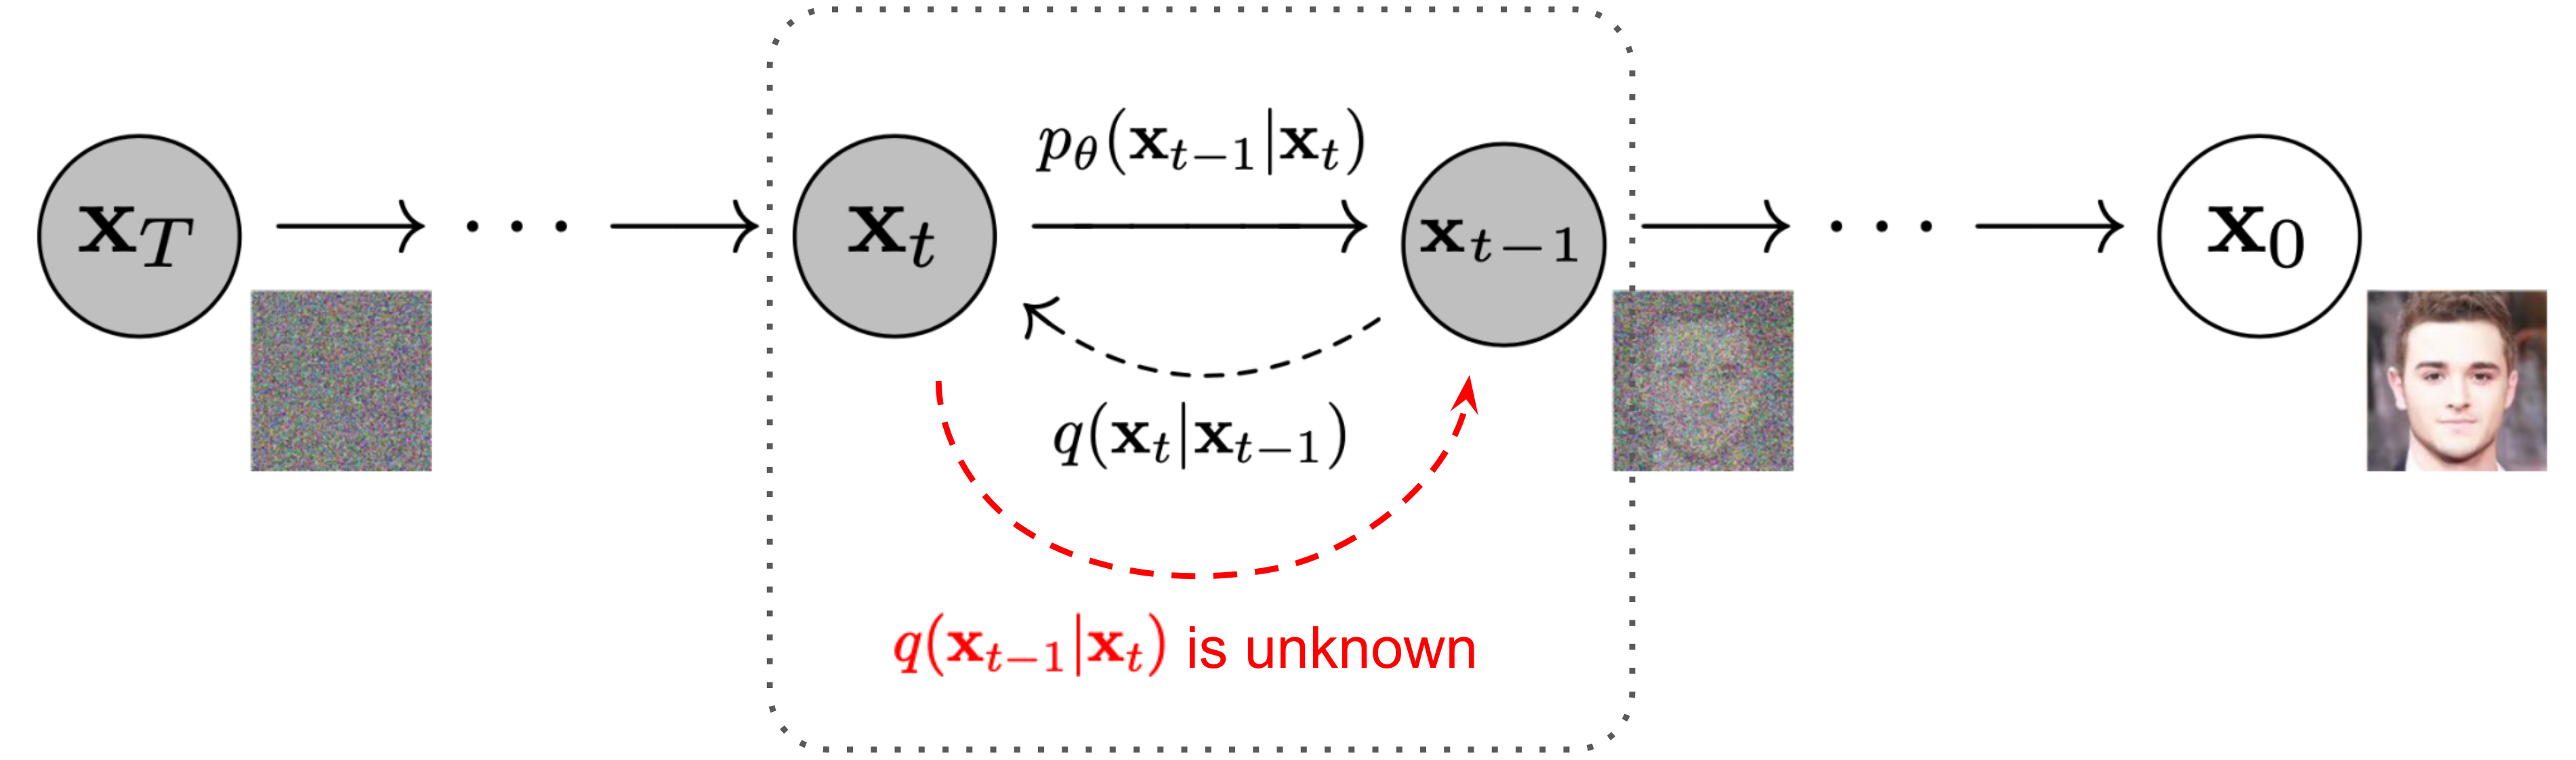
\includegraphics[width=0.8\linewidth]{figs/DDPM}
	\end{figure}
	\vspace{-0.3cm} 
	Let define the reverse process
	\vspace{-0.2cm}
	\[
		q(\bx_{t-1}|\bx_{t}) \approx p(\bx_{t - 1} | \bx_t, \btheta) = \cN \left(\bmu_{\btheta}(\bx_t, t), \bsigma_{\btheta}^2(\bx_t, t)\right)
	\]
	\vspace{-0.7cm}
	\begin{minipage}{0.5\linewidth}
		\begin{block}{Forward process}
			\begin{enumerate}
				\item $\bx_0 = \bx \sim \pi(\bx)$;
				\item $\bx_t = \sqrt{1 - \beta_t} \cdot \bx_{t - 1} + \sqrt{\beta_t} \cdot \bepsilon$, where $\bepsilon \sim \cN(0, \bI)$, $t \geq 1$;
				\item $\bx_T \sim p_{\infty}(\bx) = \cN(0, \bI)$.
			\end{enumerate}
		\end{block}
	\end{minipage}%
	\begin{minipage}{0.5\linewidth}
		\begin{block}{Reverse process}
			\begin{enumerate}
				\item $\bx_T \sim p_{\infty}(\bx) = \cN(0, \bI)$;
				\item $\bx_{t - 1} = \bsigma_{\btheta}(\bx_t, t) \cdot \bepsilon + \bmu_{\btheta}(\bx_t, t)$;
				\item $\bx_0 = \bx \sim \pi(\bx)$;
			\end{enumerate}
		\end{block}
	\end{minipage}
	\textbf{Note:} The forward process does not have any learnable parameters!
	\myfootnotewithlink{https://lilianweng.github.io/posts/2021-07-11-diffusion-models/}{Weng L. What are Diffusion Models?, blog post, 2021}
\end{frame}
%=======
\section{Gaussian diffusion model as VAE}
%=======
\begin{frame}{Gaussian diffusion model as VAE}
	\vspace{-0.2cm}
	\begin{figure}
		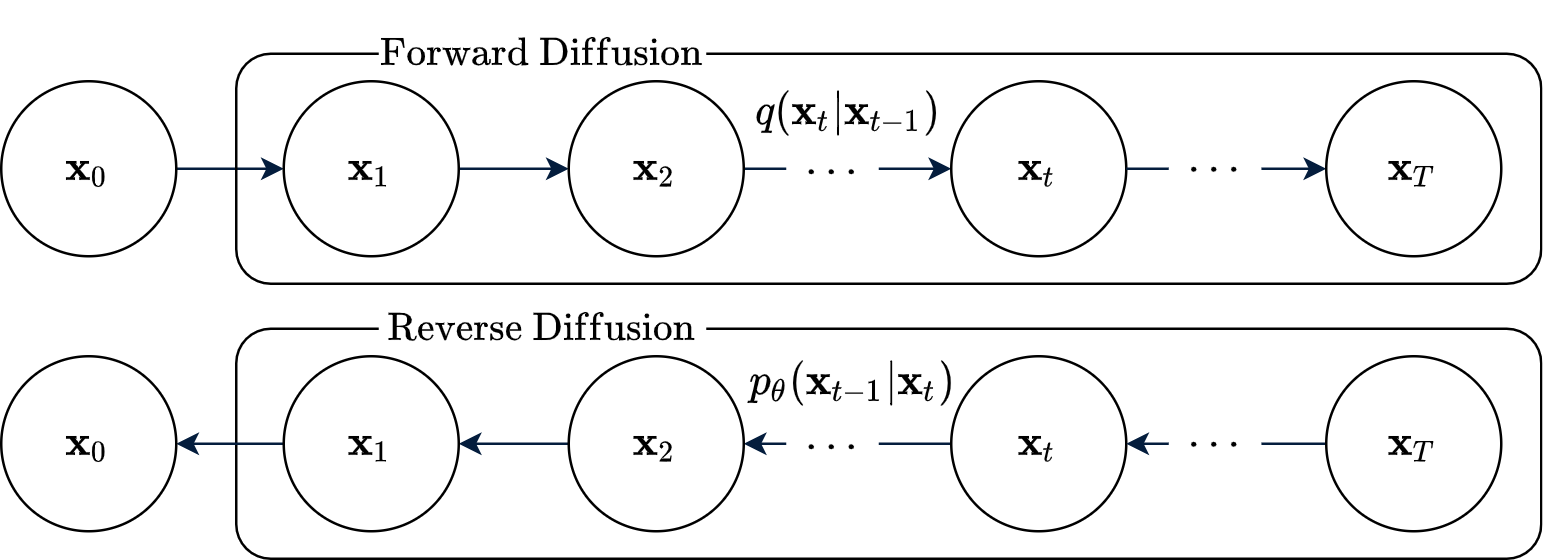
\includegraphics[width=0.65\linewidth]{figs/diffusion_pgm}
	\end{figure}
	\begin{itemize}
		\item Let treat $\bz = (\bx_1, \dots, \bx_T)$ as a latent variable (\textbf{note:} each $\bx_t$ has the same size).
		\item Variational posterior distribution (\textbf{note:} there is no learnable parameters)
		\vspace{-0.4cm}
		\[
			q(\bz | \bx) = q(\bx_1, \dots, \bx_T | \bx_0) = \prod_{t = 1}^T q(\bx_t | \bx_{t - 1}).
		\]
		\vspace{-0.5cm}
		\item Probabilistic model
		\vspace{-0.2cm}
		\[
			p(\bx, \bz | \btheta) = p(\bx | \bz, \btheta) p(\bz | \btheta)
		\]
		\item Generative distribution and prior
		\vspace{-0.3cm}
		\[
			p(\bx | \bz, \btheta) = p(\bx_0 | \bx_1, \btheta); \quad 
			p(\bz | \btheta) = \prod_{t=2}^T p(\bx_{t - 1} | \bx_t, \btheta)  \cdot p(\bx_T)
		\]
	\end{itemize}
	\myfootnotewithlink{https://ayandas.me/blog-tut/2021/12/04/diffusion-prob-models.html}{Das A. An introduction to Diffusion Probabilistic Models, blog post, 2021}
\end{frame}
%=======
\begin{frame}{ELBO for gaussian diffusion model}
	\begin{block}{Standard ELBO}
		\vspace{-0.4cm}
		\[
			\log p(\bx | \btheta) \geq \bbE_{q({\color{teal}\bz} | \bx)} \log \frac{p(\bx, {\color{teal}\bz} | \btheta)}{q({\color{teal}\bz} | \bx)} = \cL(q, \btheta) \rightarrow \max_{q, \btheta}
		\]
		\vspace{-0.5cm}
	\end{block}
	\begin{block}{Derivation}
		\vspace{-0.5cm}
		{\small
		\begin{align*}
			\cL(q, \btheta) &= \bbE_{q({\color{teal}\bx_{1:T}} | \bx_0)} \log \frac{p(\bx_0, {\color{teal}\bx_{1:T}} | \btheta)}{q({\color{teal}\bx_{1:T}} | \bx_0)} \\
			& = \bbE_{q(\bx_{1:T} | \bx_0)} \log \frac{p(\bx_T) \prod_{t=1}^T p(\bx_{t-1} | \bx_t, \btheta) }{\prod_{t=1}^T q(\bx_t | \bx_{t-1})}  \\ 
			& = \bbE_{q(\bx_{1:T} | \bx_0)} \log \frac{p(\bx_T) p(\bx_0 | \bx_1, \btheta) \prod_{t=2}^T p(\bx_{t-1} | \bx_t, \btheta) }{q(\bx_1 | \bx_0)\prod_{t=2}^T {\color{teal}q(\bx_t | \bx_{t-1})}}  \\ 
			& = \bbE_{q(\bx_{1:T} | \bx_0)} \log \frac{p(\bx_T) p(\bx_0 | \bx_1, \btheta) \prod_{t=2}^T p(\bx_{t-1} | \bx_t, \btheta) }{q(\bx_1 | \bx_0)\prod_{t=2}^T q(\bx_t | \bx_{t-1}, {\color{olive}\bx_0})} 
		\end{align*}
		}
		\[
			q(\bx_{t-1}|\bx_{t}, {\color{olive}\bx_0}) = \frac{q(\bx_{t}|\bx_{t-1}, {\color{olive}\bx_0}) q(\bx_{t-1} | {\color{olive}\bx_0}) }{q(\bx_{t}| {\color{olive}\bx_0})} = \cN(\tilde{\bmu}_t(\bx_t, \bx_0), \tilde{\beta}_t \bI)
		\]
	\end{block}
	
	\myfootnotewithlink{https://arxiv.org/abs/2006.11239}{Ho J. Denoising Diffusion Probabilistic Models, 2020}
\end{frame}
%=======
\begin{frame}{ELBO for gaussian diffusion model}
	\begin{block}{Derivation (continued)}
		\vspace{-0.7cm}
		{\small
		\begin{multline*}
			\cL(q, \btheta) = \bbE_{q(\bx_{1:T} | \bx_0)} \log \frac{p(\bx_T) p(\bx_0 | \bx_1, \btheta) \prod_{t=2}^T p(\bx_{t-1} | \bx_t, \btheta) }{q(\bx_1 | \bx_0)\prod_{t=2}^T q(\bx_t | \bx_{t-1}, {\color{olive}\bx_0})}  = \\ 
			= \bbE_{q(\bx_{1:T} | \bx_0)} \log \frac{p(\bx_T) p(\bx_0 | \bx_1, \btheta) \prod_{t=2}^T p(\bx_{t-1} | \bx_t, \btheta) }{{\color{violet}q(\bx_1 | \bx_0)}\prod_{t=2}^T \frac{q(\bx_{t-1}|\bx_t, \bx_0) {\color{violet}q(\bx_{t} | \bx_0)}}{{\color{violet}q(\bx_{t-1}| \bx_0)}}}  = \\
			= \bbE_{q(\bx_{1:T} | \bx_0)} \log \frac{{\color{violet}p(\bx_T)} {\color{olive}p(\bx_0 | \bx_1, \btheta)} \prod_{t=2}^T p(\bx_{t-1} | \bx_t, \btheta) }{{\color{violet}q(\bx_T | \bx_0)}\prod_{t=2}^T q(\bx_{t-1}|\bx_t, \bx_0)}  = \\
			= \bbE_{{\color{teal}q(\bx_{1:T} | \bx_0)}} \biggl[ \log {\color{olive}p(\bx_0 | \bx_1, \btheta)} + \log {\color{violet}\frac{p(\bx_T)}{q(\bx_T | \bx_0)}} + \sum_{t=2}^T \log \left( \frac{p(\bx_{t-1} | \bx_t, \btheta)}{q(\bx_{t-1}|\bx_{t}, \bx_0)}\right) \biggr] = \\
			 = \bbE_{{\color{teal}q(\bx_1 | \bx_0)}} \log p(\bx_0 | \bx_1, \btheta) + \bbE_{{\color{teal}q(\bx_T | \bx_0)}} \log \frac{p(\bx_T)}{q(\bx_T | \bx_0)} + \\
			  + \sum_{t=2}^T \bbE_{{\color{teal}q(\bx_{t-1}, \bx_t | \bx_0)}} \log \left( \frac{p(\bx_{t-1} | \bx_t, \btheta)}{q(\bx_{t-1}|\bx_{t}, \bx_0)}\right) 
		\end{multline*}
		}
		\vspace{-0.3cm}
	\end{block}
	\myfootnotewithlink{https://arxiv.org/abs/2006.11239}{Ho J. Denoising Diffusion Probabilistic Models, 2020}
\end{frame}
%=======
\begin{frame}{ELBO for gaussian diffusion model}
		\vspace{-0.5cm}
		\begin{multline*}
			\cL(q, \btheta) = \bbE_{q(\bx_1 | \bx_0)} \log p(\bx_0 | \bx_1, \btheta) + \bbE_{q(\bx_T | \bx_0)} \log \frac{p(\bx_T)}{q(\bx_T | \bx_0)} + \\
			  + \sum_{t=2}^T \bbE_{q(\bx_{t-1}, \bx_t | \bx_0)} \log \left( \frac{p(\bx_{t-1} | \bx_t, \btheta)}{q(\bx_{t-1}|\bx_{t}, \bx_0)}\right) =
			  \\ =  {\color{olive}\bbE_{q(\bx_1 | \bx_0)} \log p(\bx_0 | \bx_1, \btheta)} - {\color{violet}KL\bigl(q(\bx_T | \bx_0) || p(\bx_T)\bigr)} - \\
			- \sum_{t=2}^T \underbrace{ \bbE_{q(\bx_t | \bx_0)} KL \bigl(q(\bx_{t-1} | \bx_t, \bx_0) || p(\bx_{t - 1} | \bx_t, \btheta )\bigr)}_{\cL_t}
		\end{multline*}
		\vspace{-0.5cm}
	\begin{itemize}
		\item {\color{olive}First term} is a decoder distribution
		\[
			\log p(\bx_0 | \bx_1, \btheta) = \log \cN \bigl(\bx_0 | \bmu_{\btheta}(\bx_1, t), \bsigma_{\btheta}^2(\bx_1, t)\bigr).
		\] 
		\item {\color{violet}Second term} is constant ($p(\bx_T)$ is a standard Normal, $q(\bx_T | \bx_0)$ is a non-parametrical Normal).
	\end{itemize}
	\myfootnotewithlink{https://arxiv.org/abs/2006.11239}{Ho J. Denoising Diffusion Probabilistic Models, 2020}
\end{frame}
%=======
\begin{frame}{ELBO for gaussian diffusion model}
	\vspace{-0.5cm}
	\begin{multline*}
		\cL(q, \btheta) =  {\color{olive}\bbE_{q(\bx_1 | \bx_0)} \log p(\bx_0 | \bx_1, \btheta)} - {\color{violet}KL\bigl(q(\bx_T | \bx_0) || p(\bx_T)\bigr)} - \\
		- \sum_{t=2}^T \underbrace{ \bbE_{q(\bx_t | \bx_0)} KL \bigl(q(\bx_{t-1} | \bx_t, \bx_0) || p(\bx_{t - 1} | \bx_t, \btheta )\bigr)}_{\cL_t}
	\end{multline*}
	$q(\bx_{t-1} | \bx_t, \bx_0)$ defines how to denoise a noisy image $\bx_t$ with access to what the final, completely denoised image $\bx_0$ should be.
	
	\begin{figure}
		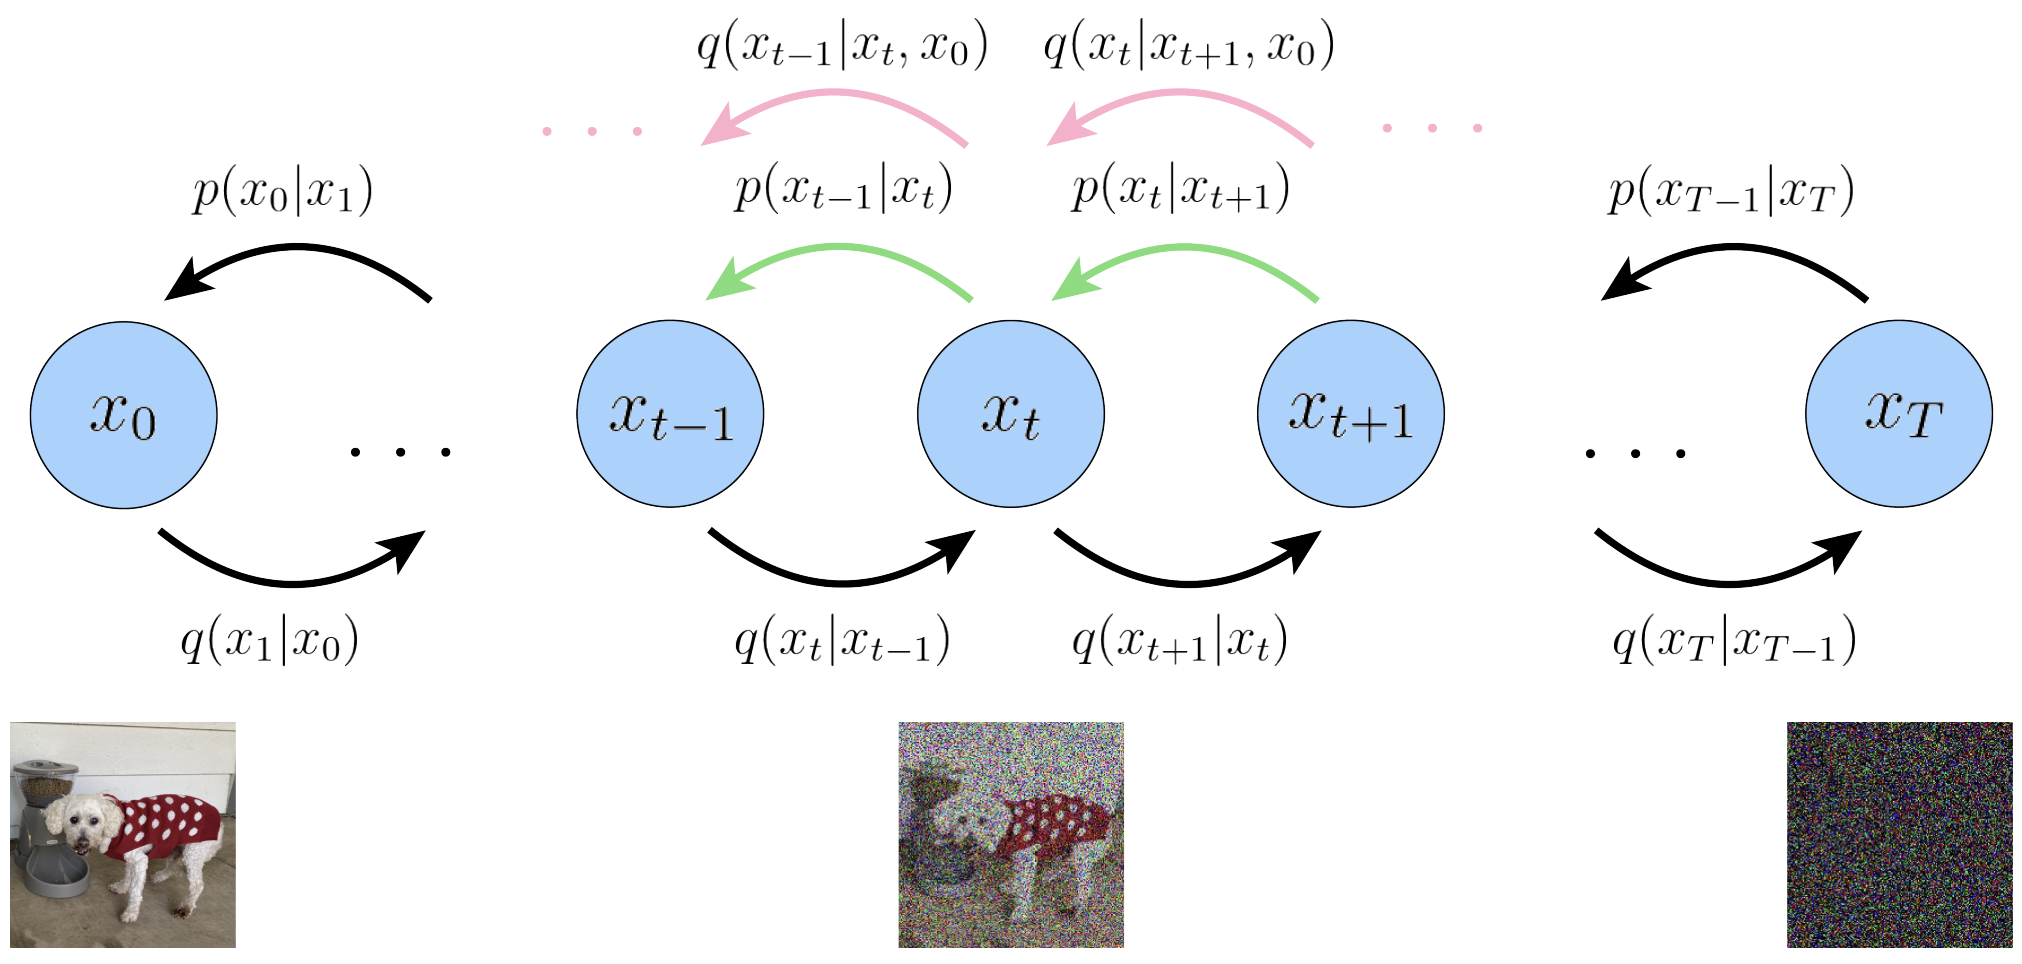
\includegraphics[width=0.85\linewidth]{figs/diffusion_objective}
	\end{figure}

	\myfootnotewithlink{https://arxiv.org/abs/2208.11970}{Luo C. Understanding Diffusion Models: A Unified Perspective, 2022}
\end{frame}
%=======
\begin{frame}{Summary}
	\begin{itemize}
		\item Gaussian diffusion process is a Markov chain that injects special form of Gaussian noise to the samples.
		\vfill
		\item Reverse process allows to sample from the real distribution $\pi(\bx)$ using samples from noise.
		\vfill
		\item Diffusion model is a VAE model which reverts gaussian diffusion process using variational inference.
		\vfill
		\item ELBO of DDPM could be represented as a sum of KL terms.
	\end{itemize}
\end{frame}
\end{document} 